\section{Результаты}

\subsection{Оценки исходной выборки} 

\begin{figure}[H]
	\begin{center}
		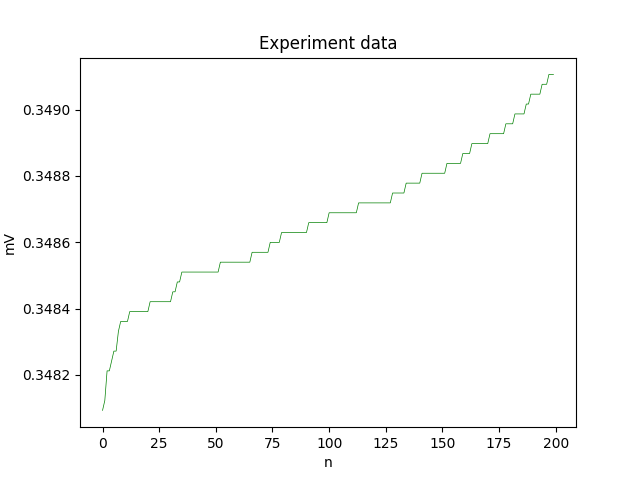
\includegraphics[scale = 0.55]{resources/data.png}
	\end{center}
	\caption{Данные выборки $\bm{X}_1$}
\end{figure}

\begin{figure}[H]
	\begin{center}
		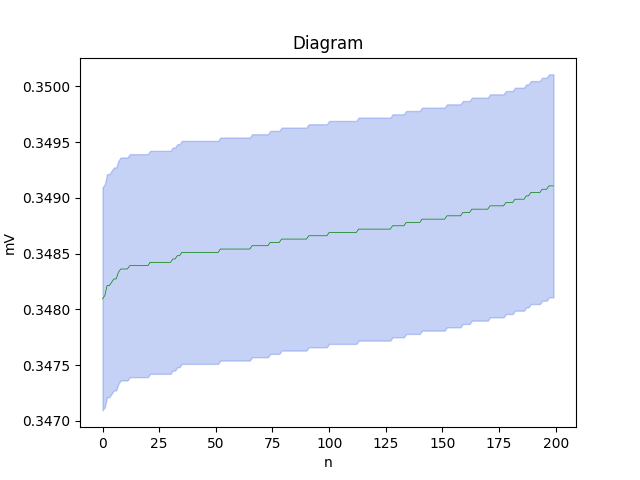
\includegraphics[scale = 0.55]{resources/diagram_beta_None.png}
	\end{center}
	\caption{Диаграмма рассеяния выборки $\bm{X}_1$ с уравновешанным интервалом неопределенности}
\end{figure}

Вычисленные внешние оценки выборки: 
\begin{equation*}
	\underline{\bm{J}}_1 = 0.34709 , \quad \overline{\bm{J}}_1 = 0.35011
\end{equation*}
\subsection{Мода и максимальная клика выборки} 

Мода выборки: 
\begin{equation*}
	\text{mode}(\bm{X}_1) = [0.34811, 0.34909]
\end{equation*}

Максимальная клика: 
\begin{equation*}
	\text{max} \mu_j (\bm{X}_1) = 200
\end{equation*}

\begin{figure}[H]
	\begin{center}
		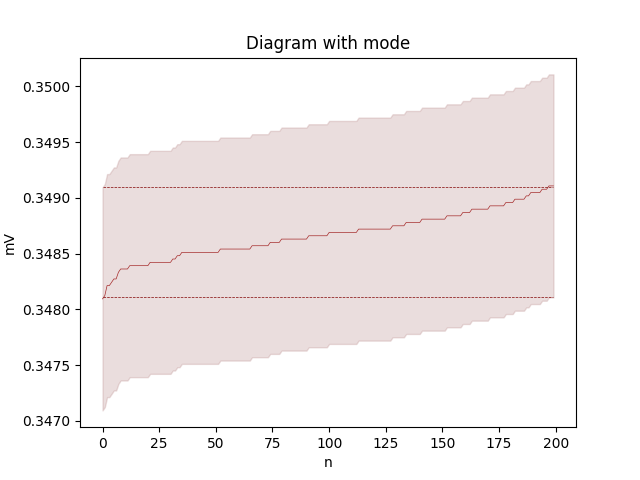
\includegraphics[scale = 0.55]{resources/diagram_with_mode.png}
	\end{center} 
	\caption{Элементы выборки $\bm{X}_1$, в которые входит мода} \label{pic:mode}
\end{figure}

\subsection{Варьирование неопределенности изменений}

В результате решения задачи линейного программирования при оптимизации по Оскорбину были найдены следующие значения: \\
Оценка постоянной: 
\begin{equation*}
	\beta = 0.34811
\end{equation*}

Коэффициент растяжения интервала неопределенности: 
\begin{equation*}
	w = 1.0
\end{equation*}

\begin{figure}[H]
	\begin{center}
		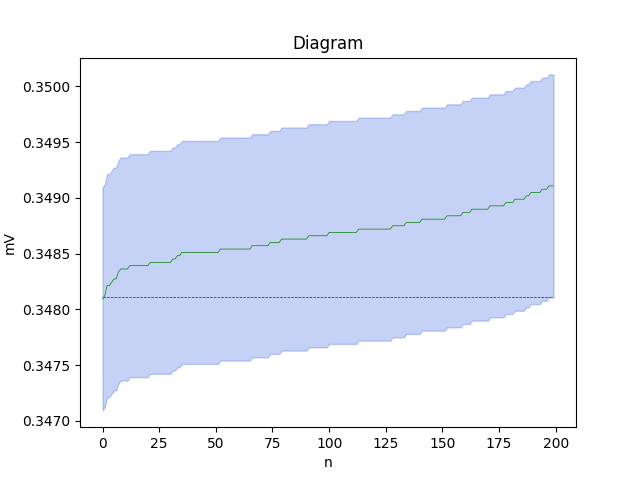
\includegraphics[scale = 0.55]{resources/diagram_beta_0.3481063.png}
	\end{center}
	\caption{Диаграмма рассеяния $\bm{X}_1$ с увеличенным в $w$ раз интервалом неопределенности}
\end{figure}

Красной пунктирной линией обозначена оценка постоянной.

\subsection{Коэффициент Жакара и относительная ширина моды}

Получены следующие значения: \\
Индекс Жакара: 
\begin{equation*}
	J_i(\bm{X}_1) = 0.32744
\end{equation*}

Относительная ширина моды: 
\begin{equation*}
	\rho(\text{mode}(\bm{X}_1)) = 0.32744
\end{equation*}

\newpage